\section{Results}
\label{sec:results}

Frozen Option~A results and labelled NEW robustness checks are never pooled.

\subsection{Accuracy and consistency are distinct (frozen)}

\paragraph{Corruption (smoke).} Gold predictions attain Acc$=$BCR$=$1. Controlled corruptions separate the metrics (Table~\ref{tab:corruption}).

\begin{table}[t]
\centering
\caption{\textbf{Frozen.} Corruption suite: Acc and BCR move independently.}
\label{tab:corruption}
\small
\begin{tabular}{lrrr}
\toprule
Corruption & Acc & BCR & $\Gapq$ \\
\midrule
high\_acc\_inconsistent & 0.849 & 0.000 & 0.849 \\
wrong\_provenance & 0.849 & 0.000 & 0.849 \\
consistent\_wrong\_world & 0.394 & 1.000 & $-$0.606 \\
transition\_inconsistency & 0.939 & 0.600 & 0.339 \\
\bottomrule
\end{tabular}
\end{table}

\paragraph{Symbolic scaled.} Retrieval baselines retain large Acc--BCR gaps (Table~\ref{tab:symbolic}; Figure~\ref{fig:accbcr}, left). B4 Acc~$=$~0.929 with BCR~$=$~0.591 ($\Gapq=0.338$). Compact flat saturates Acc/BCR at cap150 in this generator regime (fairness caveat: Section~\ref{sec:systems}).

\begin{table}[t]
\centering
\caption{\textbf{Frozen.} Symbolic scaled (102 worlds). Acc/BCR/CSR pooled point estimates (half-up, 3 decimals). Brackets: world-level bootstrap 95\% CIs for BCR/CSR.}
\label{tab:symbolic}
\small
\resizebox{\linewidth}{!}{%
\begin{tabular}{lrrrr}
\toprule
System & Acc & BCR & $\Gapq$ & mean CSR \\
\midrule
B3 recency-$k8$ & 0.567 & 0.063$_{[0.049,0.084]}$ & 0.504 & 0.507$_{[0.483,0.547]}$ \\
B4 BM25-$k8$ & 0.929 & 0.591$_{[0.586,0.596]}$ & 0.338 & 0.881$_{[0.870,0.890]}$ \\
B1 compact (cap150) & 1.000 & 1.000 & 0.000 & 1.000 \\
H0 LTKM (cap150, ret8) & 0.976 & 0.844$_{[0.820,0.898]}$ & 0.132 & 0.973$_{[0.970,0.983]}$ \\
\bottomrule
\end{tabular}}
\end{table}

\begin{figure}[t]
\centering
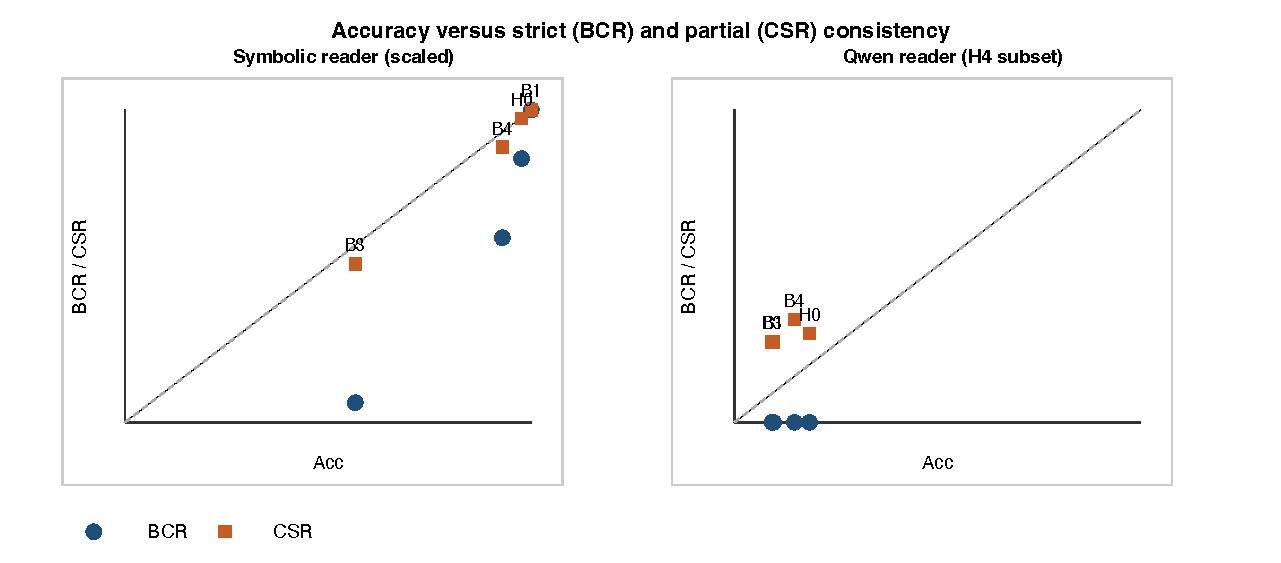
\includegraphics[width=0.95\linewidth]{figures/fig3-acc-vs-bcr-csr.pdf}
\caption{Acc vs BCR/CSR (frozen). Takeaway: Acc can remain high while BCR collapses; when BCR floors, CSR still separates systems.}
\label{fig:accbcr}
\end{figure}

\paragraph{Component ablations (frozen, symbolic H0).} Removing archive or temporal-validity components drops BCR from 0.844 to 0.375 while Acc remains 0.876 ($\Gapq=0.501$); removing graph yields Acc~$=$~0.938, BCR~$=$~0.594 (Table~\ref{tab:ablations}). These ablations localize large Acc--BCR gaps to missing lifecycle structure under the symbolic reader; they do \textbf{not} establish architectural superiority under LLM readers.

\paragraph{History-length proxy.} Acc--BCR gaps persist across small/medium/large tiers (Figure~\ref{fig:difficulty}).

\subsection{Qwen reader: BCR floors; CSR remains informative (frozen Option~A)}

On the H4 subset, all four systems have \textbf{BCR~$=$~0} (Table~\ref{tab:qwen}). Acc remains ordered (H0 0.185 highest); CSR separates B4 (0.329) from B1/B3 (0.258) and H0 (0.284). \textbf{No architecture consistency advantage is supported.}

\begin{table}[t]
\centering
\caption{\textbf{Frozen Option~A.} Qwen H4 (18 worlds, 192 bundles). All BCR~$=$~0. CSR brackets: world-level bootstrap 95\% CIs.}
\label{tab:qwen}
\small
\resizebox{\linewidth}{!}{%
\begin{tabular}{lrrrrr}
\toprule
System & Acc & BCR & mean CSR & Abs & Mal \\
\midrule
B1 compact & 0.096 & 0.000 & 0.258$_{[0.239,0.285]}$ & 0.728 & 0.007 \\
B3 recency-$k8$ & 0.093 & 0.000 & 0.258$_{[0.239,0.285]}$ & 0.728 & 0.007 \\
B4 BM25-$k8$ & 0.148 & 0.000 & 0.329$_{[0.314,0.344]}$ & 0.579 & 0.001 \\
H0 LTKM & 0.185 & 0.000 & 0.284$_{[0.275,0.298]}$ & 0.483 & 0.029 \\
\bottomrule
\end{tabular}}
\end{table}

\paragraph{Why BCR~$=$~0 is not a broken metric.} Smoke gold and symbolic systems achieve BCR~$=$~1; a labelled H4 gold re-evaluation yields Acc$=$BCR$=$1 with zero violations; under Qwen, transition fails on 192/192 bundles with mean 3.33--3.59 violations/bundle (Table~\ref{tab:violations}).

\subsection{Robustness and transfer validation (labelled NEW)}
\label{sec:robustness}

The following checks are \textbf{not} Option~A and are not merged into frozen tables.

\paragraph{Shortcut / prior baselines.} On a downsampled seed-100 protocol (18 worlds), empty answers yield Acc$=$BCR$=$0; family-wise gold-marginal majority yields Acc~$=$~0.352 with BCR~$=$~0 ($\Gapq=0.352$); family-shuffle of gold answers yields Acc~$=$~0.280 with BCR~$=$~0; gold yields Acc$=$BCR$=$1 (Table~\ref{tab:shortcuts}). Non-zero Acc with BCR~$=$~0 under marginal/shuffle controls shows BCR is not a rebranding of Acc.

\paragraph{Seeds.} Symbolic B3/B4 at $k{=}8$, 6 worlds/tier, seeds 100--105: B3 $\Gapq=0.504$ on every seed; B4 $\Gapq\in[0.335,0.338]$ (Table~\ref{tab:seeds}). Seed diversity is limited under this template-heavy generator (B3 identical; B4 Acc varies only slightly); we report this limitation rather than claim broad seed robustness.

\paragraph{Relation density / distractors.} On 8 medium worlds (seed base 200), varying relation density $\{0,0.2,0.5,0.8,1.0\}$ preserves large B4 gaps ($\Gapq\in[0.309,0.317]$) with BCR~$=$~0.600. Toggling distractors on seed-100 with 6 worlds/tier leaves B3/B4 Acc and BCR unchanged under the symbolic reader (null result; Table~\ref{tab:density}).

\paragraph{Stronger LLM readers.} Not completed in this environment (\texttt{mlx\_lm} unavailable; limited disk). Option~A remains a single 3B Qwen reader.
